\subsection{Bilkontrol}
\figOC{Diagrammer/BDDBilkontrol.eps}{1}{Diagram der viser de forskellige elementer i bilkontrollen og selve controllerenhederne.}

\subsubsection*{\textbf{Bilkontrol}}
Bilkontrollen er den centrale enhed som samler input fra controllere, sender signal til de to bots om retning og hastighed og styrer spillet. 
\subsubsection*{\textbf{Embedded controller}}
Bilkontrollens software eksekveres på en embedded controller med Linux-system. 
\subsubsection*{\textbf{Receiver}}
Receiver-modulet modtager serielt ikke-processeret input fra controllerens joystik og mikrofon via kabel. 
\subsubsection*{\textbf{Transmitter}}
Transmitter-modulet varetager den trådløse forbindelse til de to bots.
\subsubsection*{\textbf{Trådløs IF}}
Trådløse interface-modulet fungerer som undermodul til Transmitter-modulet og varetager den trådløse forbindelse til de to bots. 
\subsubsection*{\textbf{Digital lydbehandling}}
Digital lydbehandlings-modulet processerer mikrofonernes inputs således disse kan indgå i gameplayet som en styring til de to bots.  
\subsubsection*{\textbf{Gameplay}}
Gameplay-modulet varetager styring af spillets gang mv.  
\subsubsection*{\textbf{Point}}
Point-undermodulet til gameplay-modulet styrer spillernes point 
\subsubsection*{\textbf{Display}}
Display-undermodulet til gameplay-modulet viser kampens status igennem spillernes point. 
\subsubsection*{\textbf{Controller behandling}}
Controller behandlingsmodulet omsætter de ikke-processerede input fra controlleren (herved forstås input fra joystik og mikrofon) og omsætter dem til retning og hastighed for de to bots.  
\subsubsection*{\textbf{Joystick behandling}}
Joystick behandlingsmodulet omsætter det ikke-processerede input fra joystikket til retning og hastighed for de to bots.

\begin{figure*}
	\centering
   	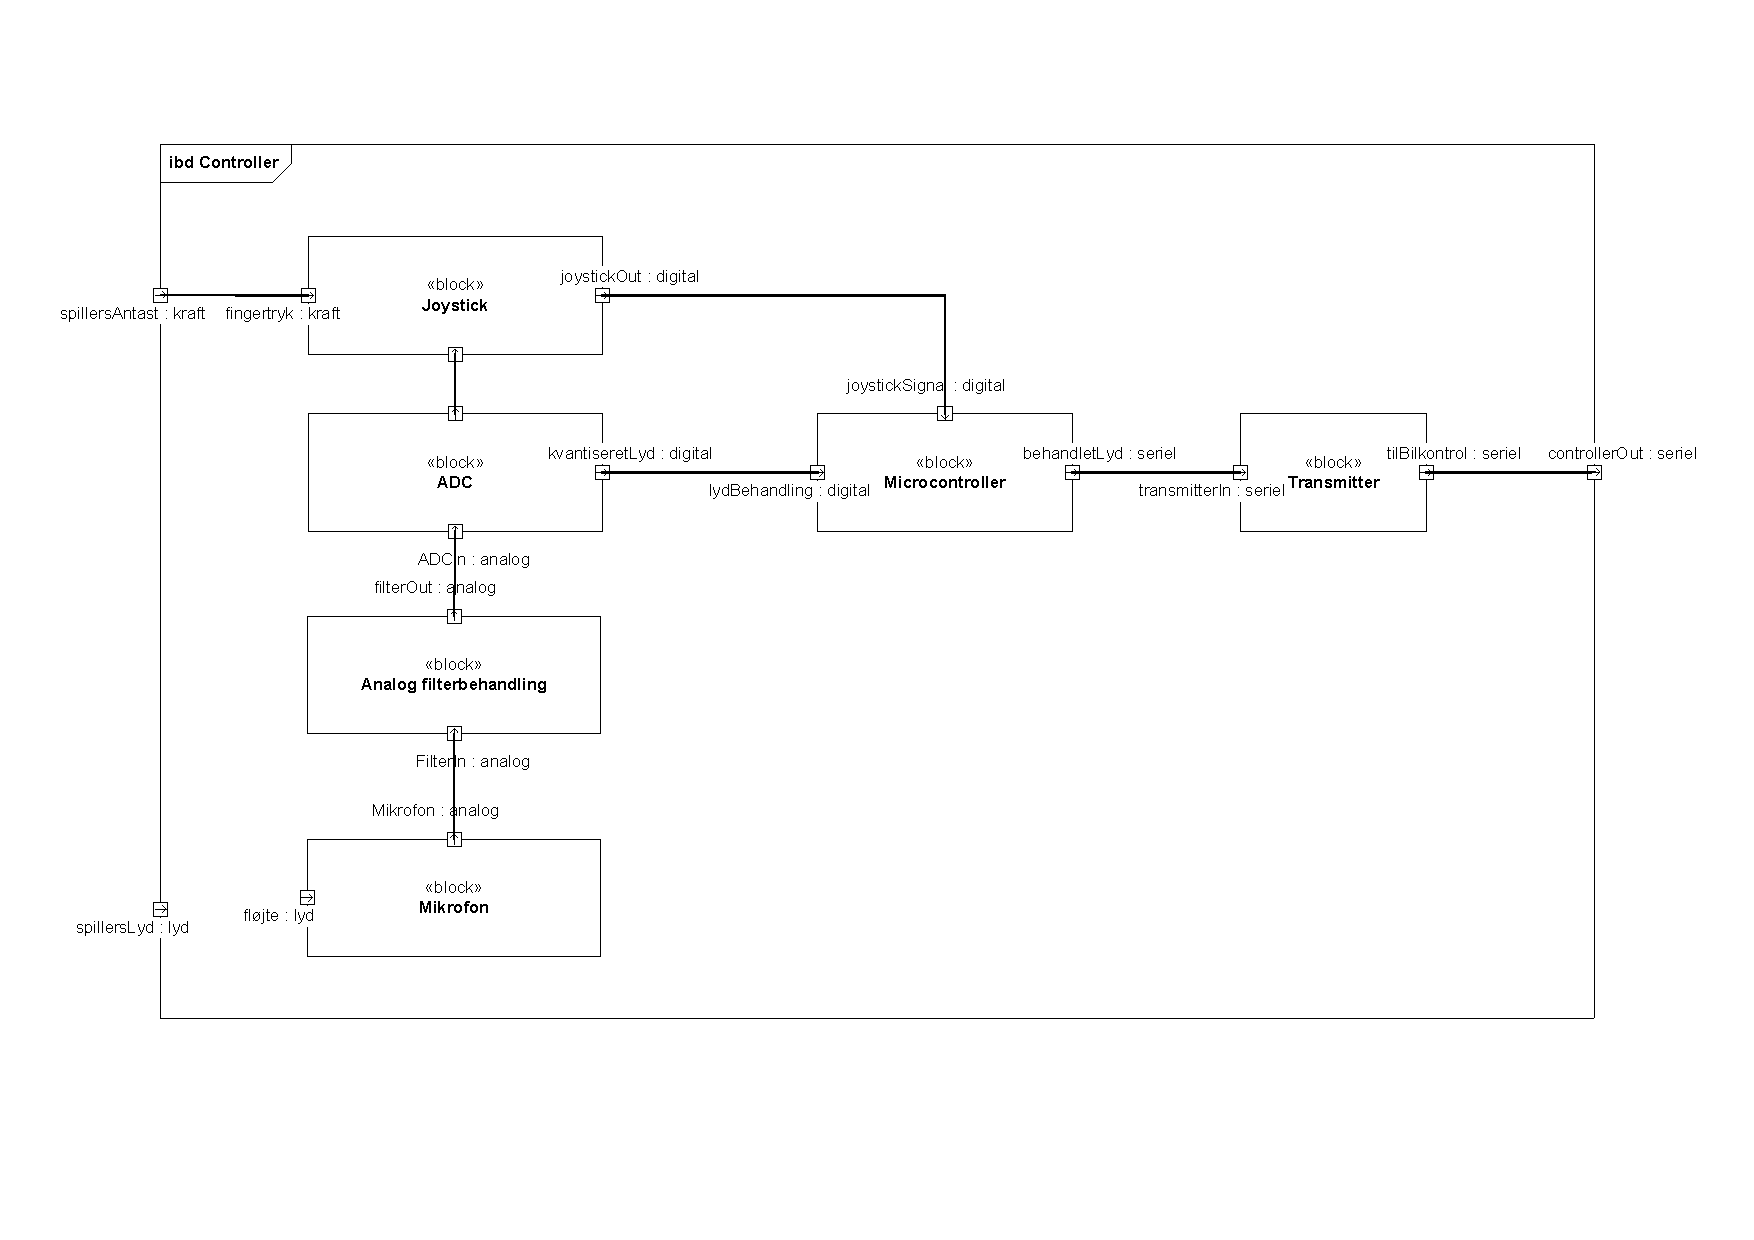
\includegraphics[page=1,width=1\linewidth]{figs/Diagrammer/IBD_SumoBot_BilKontrol_Controller.pdf}
	\caption{IBD for Controller}
	\label{fig:IBD_Controller}
\end{figure*}
\begin{figure*}
	\centering
   	\includegraphics[page=2,width=1\linewidth]{figs/Diagrammer/IBD_SumoBot_BilKontrol_Controller.pdf}
	\caption{IBD for Bilkontrol}
	\label{fig:IBD_Bilkontrol}
\end{figure*}
\begin{figure*}
	\centering
   	\includegraphics[page=3,width=1\linewidth]{figs/Diagrammer/IBD_SumoBot_BilKontrol_Controller.pdf}
	\caption{IBD for SumoBot}
	\label{fig:IBD_SumoBot}
\end{figure*}

\subsection{Kontroller}
\subsubsection*{\textbf{Controller}}\hfill\\
Controller udgøre grænsefladen til den fysiske værden. Her konvertere force og lyd til data som bilkontrol kan læse og respondere på.
\subsubsection*{\textbf{Microcontroller}}\hfill\\
Microcontroller står for alt modtagelse af analoge signaler fra henholdsvis lydmodul og Joystick, oversætter det til data, som derfra sendes til Bilkontrold via transmitteren.
\subsubsection*{\textbf{Transmitter}}\hfill\\
Kommunikations portal til bilkontrol.
\subsubsection*{\textbf{ADC}}\hfill\\
Oversætter analoge signaler til digitale.
\subsubsection*{\textbf{Joystick}}\hfill\\
Joystic oversætter force til spændinger, som kan læses af microcontrolleren.
\subsubsection*{\textbf{Lyd-modul}}\hfill\\
Lydmodul konvertere lyd til analoge signaler som microcontrolleren kan evaluere på.
\subsubsection*{\textbf{Mikrofon}}\hfill\\
mikrofon gør det muligt for systemet at modtage lyd fra omverdenen.
\subsubsection*{\textbf{Analog filterbehandling}}\hfill\\
Analog filterbehandling filtrerer uønsket frekvenser modtaget fra mikrokrofonen og forstærker eller formindsker signalet, således det er læsbart for en mikrocontroller.